This chapter reports the empirical work already completed. Three studies are
described in sequence. The first two are ordered from the most controlled to the
most demanding setting: a small, balanced experiment with handcrafted texture
descriptors, and a large-scale experiment with deep convolutional models over
hundreds of thousands of minimaps. The third isolates a single question that the
proposal depends on, whether anonymization costs predictive performance, and
answers it with a paired design and an explicit statistical statement. The
chapter then consolidates what the studies jointly support, maps that evidence
back to the research questions, and is explicit about the limitations that
prevent the current results from being read as final. The research plan of
Chapter~\ref{chapter:research-plan} is built to resolve them.

\section{Role of Preliminary Studies}

This chapter consolidates the empirical evidence already produced during the
doctoral research. The goal is not to present the final thesis results, but to
show that the proposed direction is viable and that the remaining work is built
on concrete artifacts. Two studies are central. The first evaluates source code
minimaps with Local Binary Patterns and traditional machine learning
\cite{gebara2025iwssip}. The second scales the approach to hundreds of thousands
of minimaps and evaluates deep learning models with explainability
\cite{gebara2025ciarp}. A third study isolates the anonymization question with a
paired design.

Together, these studies support four claims. First, source code minimaps encode
discriminative information about software artifacts. Second, both handcrafted
texture descriptors and learned visual representations can exploit this
information. Third, explainability methods can reveal which visual regions
models use when making predictions. Fourth, suppressing lexical content does not
cost predictive performance in the setting where this has been measured, even
though it removes more than half of the information carried by each pixel.

\section{Study 1: Feature Detection with Texture Descriptors}

The first study introduced source code minimaps as visual signatures for
software feature detection \cite{gebara2025iwssip}. The methodology generated
minimap images from source files, applied anonymization, extracted Local Binary
Pattern histograms, and trained traditional classifiers. The evaluated models
included K-Nearest Neighbors, Random Forest, and Support Vector Machines.

The study was motivated by the observation that software artifacts often have
visual texture. Some classes contain repeated fields and annotations, some test
files contain repeated assertions and setup methods, some front-end files contain
dense markup, and some configuration files contain short nested structures.
Instead of manually defining rules for each stereotype, the study asked whether
these visual patterns could be learned from minimap images.

Figure~\ref{fig:lbp} illustrates the Local Binary Pattern operator used as the
texture descriptor.

\begin{figure}[ht]
    \centering
    \caption{Local Binary Pattern operator used for texture extraction.}
    \label{fig:lbp}
    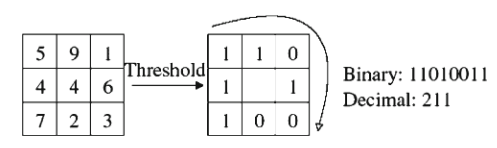
\includegraphics[width=0.70\textwidth]{figuras/lbp.png}
    \fadaptada{martins2013database}
\end{figure}

The operator works as follows \cite{ojala2002lbp}. Each pixel of the image is
taken in turn as the center of a neighborhood, and its intensity is used as a
local threshold. Every neighbor is compared with the center and replaced by a
single bit: one if the neighbor is greater than or equal to the center, zero
otherwise. In the example of Figure~\ref{fig:lbp}, the center value 4 converts
the surrounding intensities into the bits shown in the middle grid. Reading
these bits in a fixed circular order produces a binary word, here 11010011,
whose decimal value 211 becomes the code assigned to that pixel. Two parameters
control the operator: the number of sampled neighbors and the radius of the
circle on which they lie, which together determine the spatial scale of the
pattern being described.

Applying this procedure to every pixel yields a code image, and the descriptor
of the minimap is the histogram of those codes. Taking the histogram is the step
that makes the representation useful: it discards where each pattern occurred
and retains only how often each local configuration appears, so two files with the same
layout conventions produce similar descriptors even when their content differs.
The study used eight sampling points on a radius of two pixels and the
non-rotation-invariant uniform variant of the operator, which keeps every
uniform pattern, i.e., every code with at most two bit transitions in the
circular word, as an individual bin and collapses the remaining codes into a
single bin. This yields a descriptor of 59 bins per minimap, normalized to sum
to one so that images of different sizes remain comparable.

Two properties explain why this operator is a reasonable first choice for
minimaps. It is invariant to monotonic changes in overall intensity, because
only comparisons between neighbors matter, and it responds to exactly the kind
of structure a minimap encodes: indentation steps, line endings, and dense
punctuation regions all appear as recurring local intensity transitions rather
than as objects with semantic boundaries.

The study generated two dataset variants. The first used variable-size minimaps,
where image dimensions reflected source file dimensions. The second used
fixed-size minimaps, especially 128 by 128 pixels, to support later comparison
with neural image models. This distinction is important because variable-size
minimaps preserve more original layout information, while fixed-size minimaps
simplify modeling.

\subsection{Dataset and Classes}

The initial dataset was generated from two large private software projects, made
available under a confidentiality agreement: an enterprise resource planning
system from a company in the industrial sector, and a system developed by the
Brazilian federal government. Their size and heterogeneity made them a realistic
basis for the study, and they could only be used because anonymization removed
the lexical layer. Processing them produced 42,820 minimap images, organized into 28
classes representing file types and Java-related stereotypes, including Java
entities, repositories, services, unit tests, JavaScript files, JSON files, SVG
files, XML files, properties files, shell scripts, and SQL files. The complete
raw class distribution was imbalanced, with some classes containing only a few
instances and others containing thousands.

One implementation detail of the generation step affects the descriptor. An
eight-pixel dead zone was added around every image in both dataset variants, so
that the LBP operator can be evaluated on pixels near the original borders
without discarding them.

For the first controlled evaluation, the study kept only classes with more than
1,000 examples and drew exactly 1,000 random samples from each, which yields a
balanced setting. This produced seven classes: JSON, SVG, JavaScript, JSP, and
the Java stereotypes Entity, UnitTest, and ServiceImplementation. The design
provided a controlled scenario in which to test whether the representation
itself contained useful visual signals.

The published article does not report the partitioning scheme, so the protocol
described here was recovered from the accompanying artifact repository and
should be read as a reconstruction. Classes are capped as described above and
the resulting descriptor matrix is split once into 80\% training and 20\% test
partitions under a fixed random seed. Hyperparameters for each classifier are
selected by grid search with five-fold cross-validation over the training
partition only, and the test partition is used exclusively for the reported
figures. Two limitations of this protocol should be stated explicitly. The split
is not stratified by class label, so balance in the test partition follows from
the sampling cap rather than from the splitting procedure itself; and because a
single split is used, the reported values carry no variance estimate. Recording
the protocol explicitly and repeating the evaluation over multiple seeds is part
of the planned work described in Chapter~\ref{chapter:research-plan}.

Figure~\ref{fig:lbp-histograms} presents average LBP histograms for six
representative classes, computed over 1{,}000 minimaps per class. The figure is
split into two panels because the descriptor has a strongly skewed shape. Two
codes dominate every class: the code produced by a flat neighborhood and the
catch-all bin for non-uniform patterns. Together they account for between 91\%
and 99\% of the mass, which is expected, since a minimap is mostly empty
background. The upper panel shows the complete descriptor on a logarithmic
scale so that this dominance is visible; the lower panel restricts the view to
the remaining codes on a linear scale, where the classes actually separate.

\begin{figure}[ht]
    \centering
    \caption{Average LBP histograms for six minimap classes. Upper panel:
    complete descriptor, logarithmic scale. Lower panel: codes 0--56, linear
    scale.}
    \label{fig:lbp-histograms}
    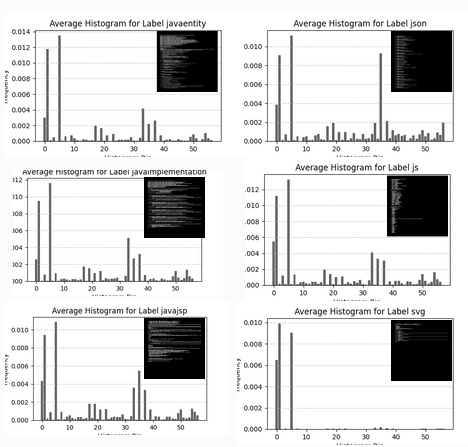
\includegraphics[width=0.92\textwidth]{figuras/lbp-histograms.png}
    \fautor
\end{figure}

Read this way, the figure carries a more precise message than a claim of visual
similarity. The discriminative structure occupies a small fraction of the
descriptor, from 0.4\% of the mass for SVG files to 7.5\% for JSP pages, and it
is concentrated in a few codes that correspond to horizontal and vertical
intensity transitions, i.e., to line endings and indentation steps. The classes
separate mostly by how much of that structure they contain and in which
proportion. SVG files are an instructive case: their minimaps are almost
entirely flat, so their descriptor is nearly degenerate, yet this very emptiness
makes them trivially separable from every other class. Java entity and Java
implementation files, in contrast, produce nearly superposed profiles, which
anticipates the confusion observed between them in the results below.

\subsection{Results}

Table~\ref{tab:study1-results} summarizes the main performance results reported
for the three traditional classifiers. The published study reports a single
figure of merit, overall accuracy on the test partition, and the table therefore
reports that quantity alone.\footnote{Earlier versions of this table presented
the same value under three separate headings for precision, recall, and
F1-score. That presentation was misleading: no per-class or averaged
precision-recall figures were computed for this experiment. Producing them, from
the per-class classification reports that the pipeline already generates, is
part of the consolidation work described in
Chapter~\ref{chapter:research-plan}.} The values should be interpreted as
preliminary evidence, both because the dataset was limited when compared with
the later large-scale corpus and because accuracy alone says nothing about how
the errors are distributed across classes.

\begin{table}[ht]
\centering
\caption{Summary of preliminary results with LBP features.}
\label{tab:study1-results}
\begin{tabular}{p{0.34\textwidth}c}
\toprule
\textbf{Classifier and dataset} & \textbf{Accuracy} \\
\midrule
KNN, variable-size minimaps & 0.79 \\
KNN, fixed-size minimaps & 0.78 \\
Random Forest, variable-size minimaps & 0.93 \\
Random Forest, fixed-size minimaps & 0.93 \\
SVM, variable-size minimaps & 0.89 \\
SVM, fixed-size minimaps & 0.88 \\
\bottomrule
\end{tabular}
\fautor
\end{table}

Random Forest achieved the best overall results, reaching approximately 93\%
accuracy in both fixed-size and variable-size settings. This result is
important because it indicates that minimap texture contains discriminative
signals even before using deep learning. SVM also performed strongly, while KNN
was less effective, suggesting that the feature space benefits from models that
can learn more complex decision boundaries or ensemble combinations. Across all
three classifiers the variable-size minimaps are equal or marginally superior to
the fixed-size ones, by at most one percentage point, which is consistent with
the fact that resizing to 128 by 128 pixels discards layout information. The
margin is small enough that fixed-size minimaps remain the sensible choice for
the convolutional experiments that follow, where a uniform input size is
required.

Figure~\ref{fig:confusion-rf} shows the confusion matrices for Random Forest in
the fixed-size and variable-size settings. The matrices indicate strong
performance for visually distinctive classes such as JSON and SVG, while some
Java-related classes exhibit more confusion because they share structural
similarities.

\begin{figure}[ht]
    \centering
    \caption{Random Forest confusion matrices for fixed-size and variable-size minimaps.}
    \label{fig:confusion-rf}
    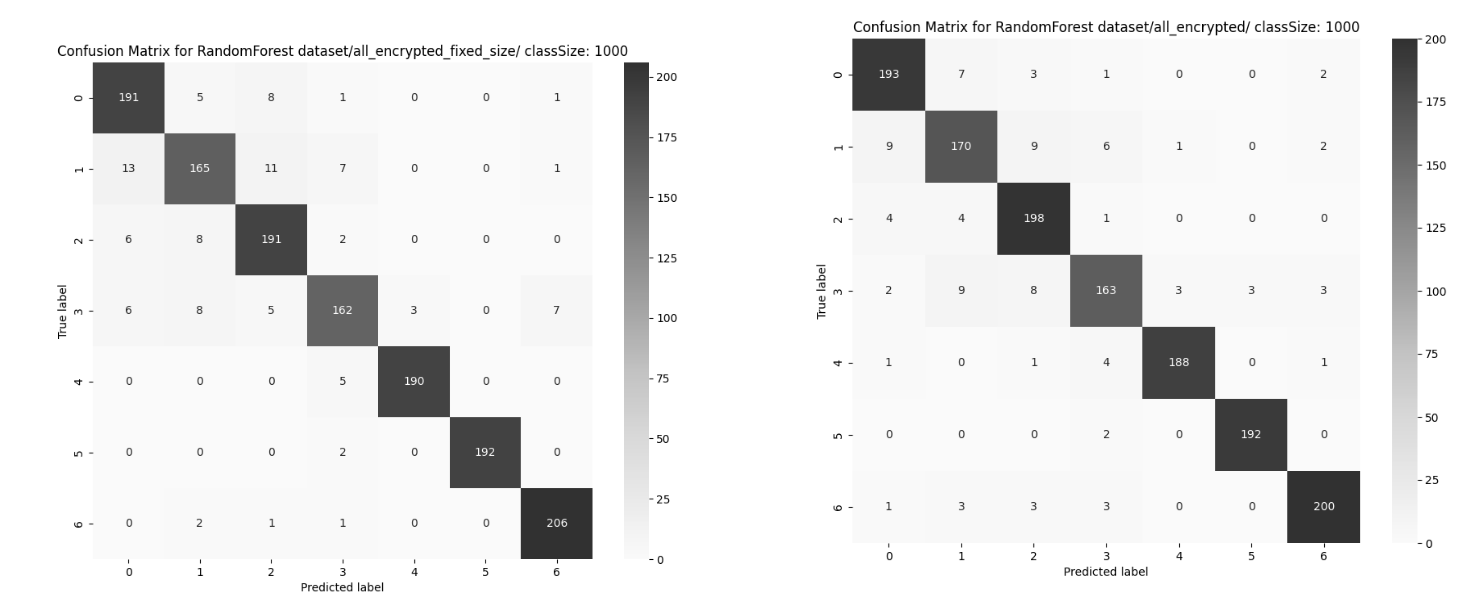
\includegraphics[width=0.92\textwidth]{figuras/confusion-rf.png}
    \fautor
\end{figure}

\subsection{Lessons from Study 1}

The first study produced four lessons that guide the rest of the doctorate.
First, source code minimaps can support classification without relying on
language-specific parsers. Second, anonymization did not prevent the models from
learning useful visual patterns in the evaluated setting. Third, fixed-size
minimaps remained competitive with variable-size minimaps, making them suitable
for convolutional models. Fourth, class similarity matters: files with similar
roles and layouts may be difficult to separate with texture descriptors alone.

These lessons motivated the second study. If minimaps work with handcrafted
features in a limited setting, the next question is whether they scale to more
projects, languages, classes, and learning objectives.

\section{Study 2: Large-Scale Deep Learning}
\label{sec:study2}

The second study expanded the evaluation to a large-scale corpus of source code
minimaps \cite{gebara2025ciarp}. The dataset contains 685,906 minimap images
extracted from 100 open-source projects across 10 programming languages. The
images are standardized to 128 by 128 pixels and accompanied by a file-level
catalog. The study evaluates three objectives: Type, Project, and Author.

The scale of the dataset changes the nature of the problem. Instead of asking
whether a few visually distinct classes can be separated, the study asks whether
minimaps preserve useful information across many repositories and heterogeneous
ecosystems. It also introduces severe class imbalance, especially because some
projects and file types are much more frequent than others.

Figure~\ref{fig:dist-type} presents the distribution of the top Type classes,
while Figures~\ref{fig:dist-project} and \ref{fig:dist-author} present the top
Project and Author classes.

\begin{figure}[ht]
    \centering
    \caption{Top Type classes in the large-scale minimap dataset.}
    \label{fig:dist-type}
    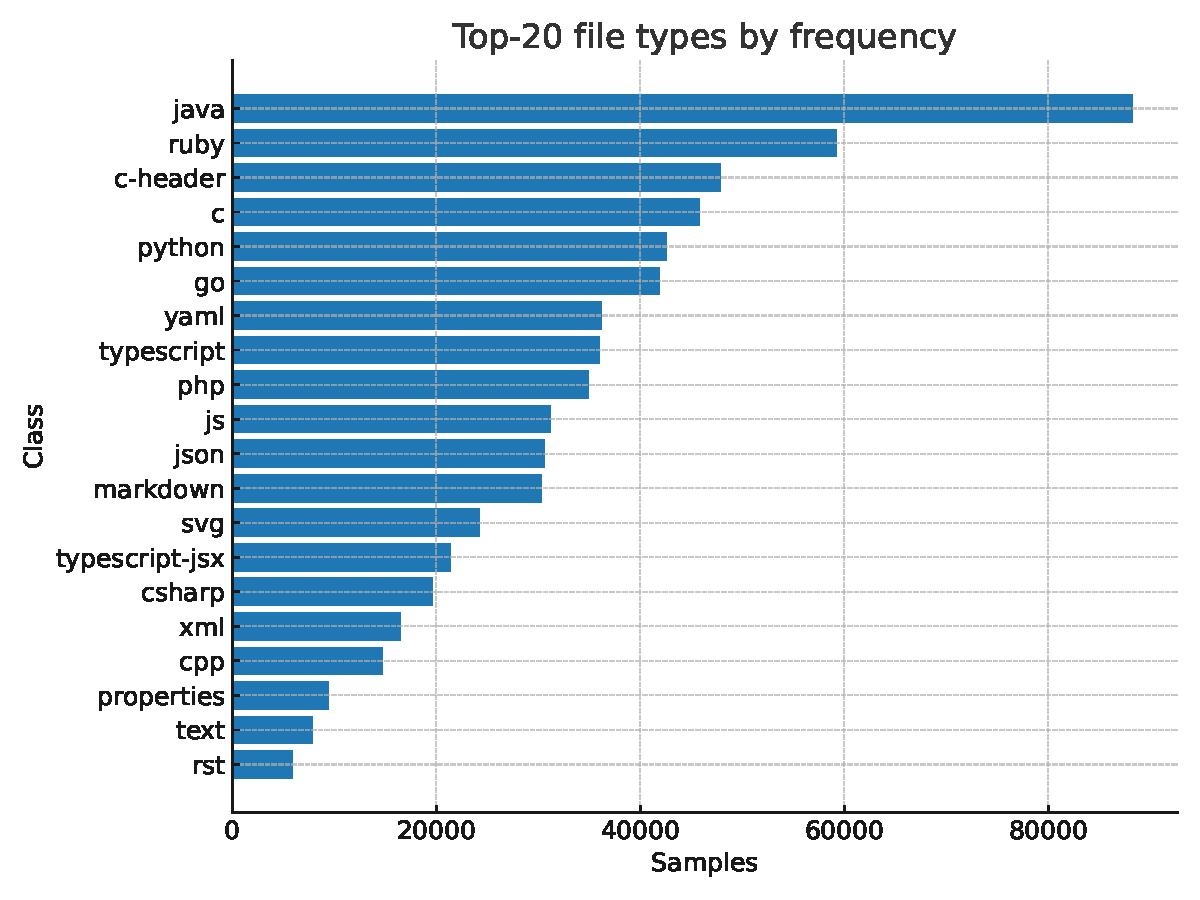
\includegraphics[width=0.82\textwidth]{figuras/dist-type-top20.pdf}
    \fautor
\end{figure}

\begin{figure}[ht]
    \centering
    \caption{Top Project classes in the large-scale minimap dataset.}
    \label{fig:dist-project}
    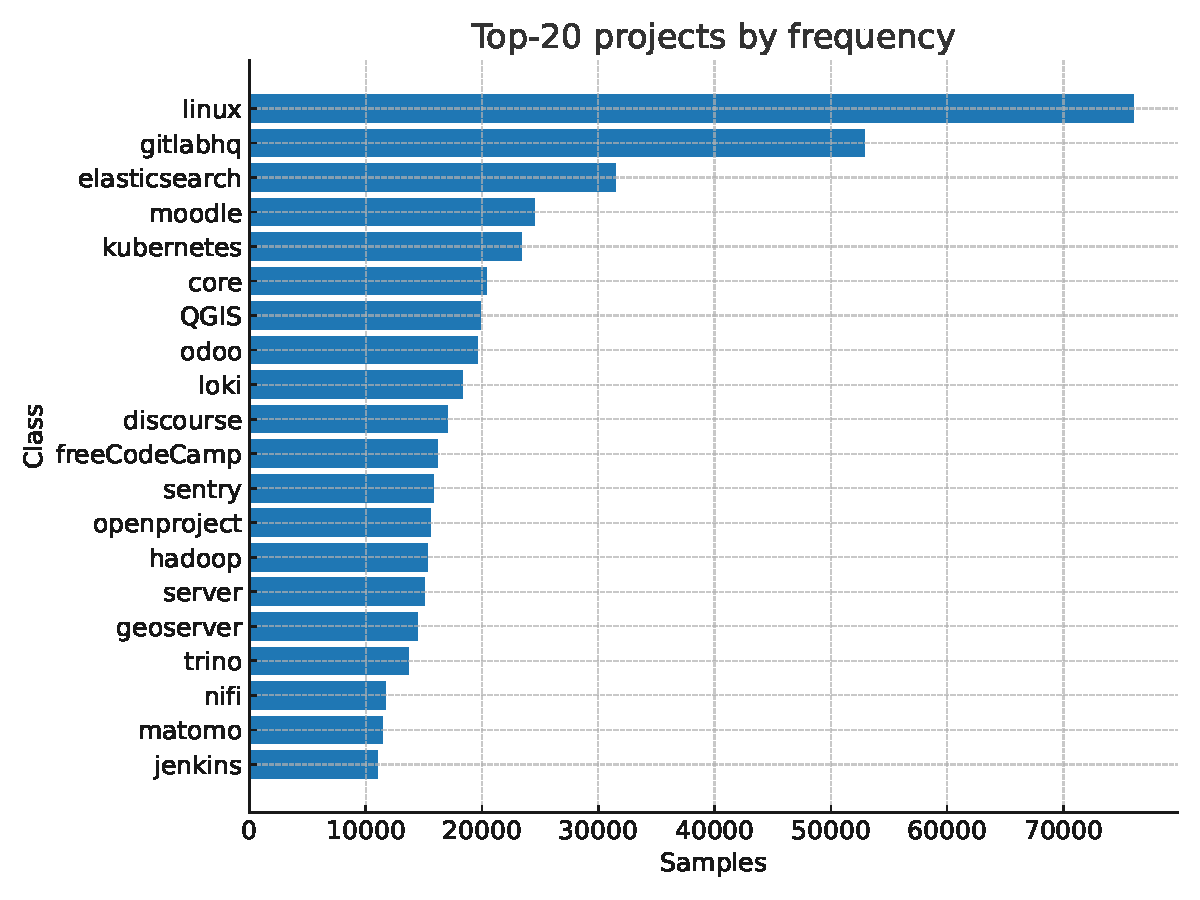
\includegraphics[width=0.82\textwidth]{figuras/dist-project-top20.pdf}
    \fautor
\end{figure}

\begin{figure}[ht]
    \centering
    \caption{Top Author classes in the large-scale minimap dataset.}
    \label{fig:dist-author}
    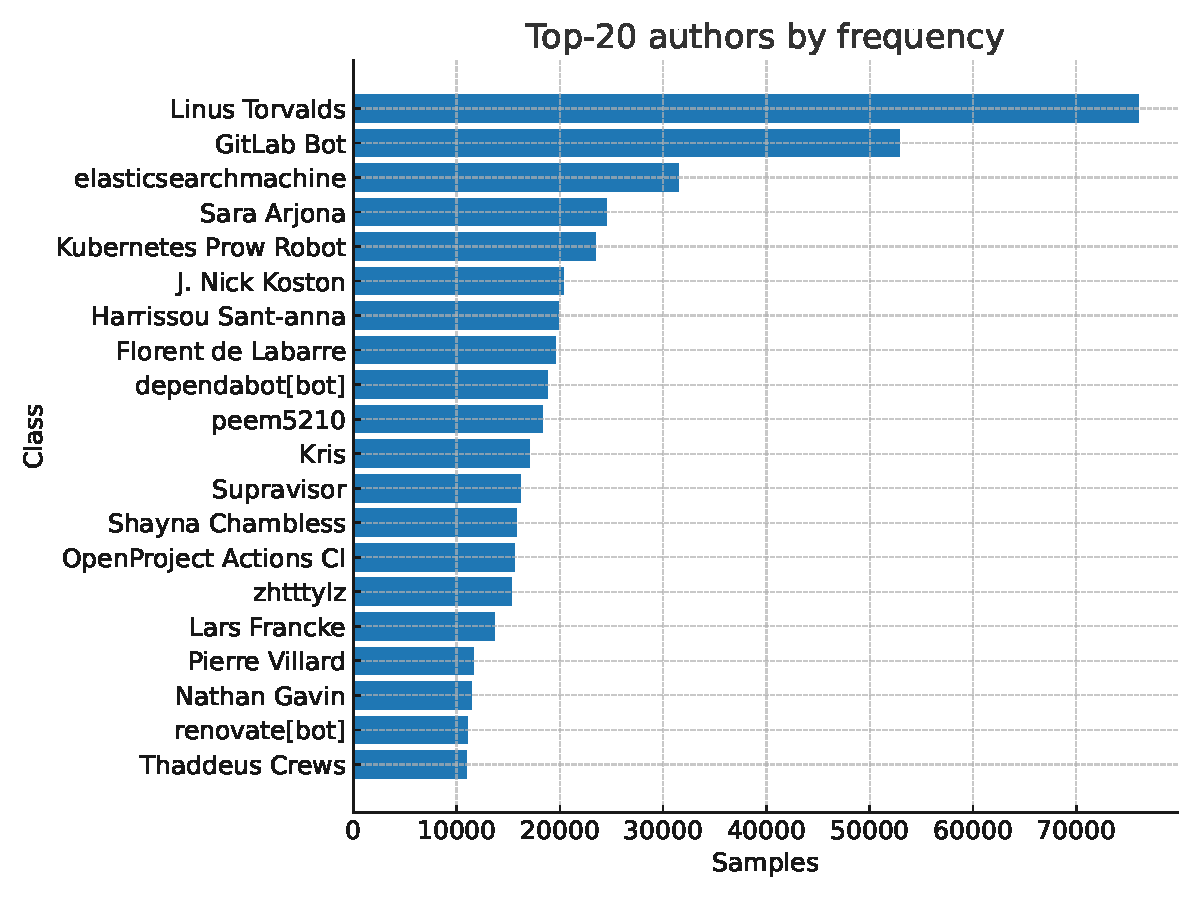
\includegraphics[width=0.82\textwidth]{figuras/dist-author-top20.pdf}
    \fautor
\end{figure}

\subsection{Dataset Summary}

Table~\ref{tab:study2-dataset} summarizes the main dataset statistics. The
numbers show that the corpus is large enough to train deep models, but also
imbalanced enough to require careful evaluation.

\begin{table}[ht]
\centering
\caption{Summary of the large-scale minimap dataset.}
\label{tab:study2-dataset}
\begin{tabular}{lr}
\toprule
\textbf{Property} & \textbf{Value} \\
\midrule
Number of minimap images & 685,906 \\
Number of open-source projects & 100 \\
Number of programming languages & 10 \\
Type classes & 63 \\
Project classes & 99 \\
Author classes & 97 \\
Default image size & 128 by 128 pixels \\
Default color mode & Grayscale \\
\bottomrule
\end{tabular}
\fautor
\end{table}

The Type objective contains file-role categories such as programming-language
files, headers, configuration formats, markup, scripts, and other artifacts. The
Project objective reflects repository identity.\footnote{The corpus was
generated from 100 repositories, while the label catalog records 99 distinct
Project classes. Documenting the precise origin of this one-class difference is
part of the dataset-curation activity (A1) in
Chapter~\ref{chapter:research-plan}.} The Author objective reflects
last-committer or author labels as recorded by the dataset-generation process.
Because this objective may conflate humans, bots, and organizational accounts,
it is interpreted cautiously.

\subsection{Training Protocol}

The large-scale study evaluates convolutional backbones under a unified
protocol. Inputs are fixed-size 128 by 128 grayscale minimaps. Models are
trained with early stopping and evaluated using accuracy and ROC-AUC, with
macro-F1 and weighted-F1 used to interpret class imbalance. The evaluated
architectures are ResNet-18 and EfficientNet-B0, tested in two
configurations: trained from scratch on the minimap corpus, and initialized
from ImageNet pretrained weights followed by fine-tuning
\cite{he2016resnet,tan2019efficientnet}. Vision Transformer configurations
(ViT-B/16) were also exercised during early experimentation, but the
consolidated evaluation focused on the two convolutional backbones; a
systematic transformer comparison is deferred to the research plan.

Three details of the data protocol matter for interpreting the results. Before splitting, classes with
fewer than 100 samples were excluded and classes were capped at 5,000 samples,
which limits extreme imbalance but also means that the effective number of
classes seen by the models can be smaller than the catalog totals. The data
were then split at file level into 70\% training, 15\% validation, and 15\%
test partitions, stratified by class label and controlled by a fixed random
seed. The split is not repository-disjoint: files from the same project can
appear in different partitions. For the Project objective this is unavoidable,
since each project is itself a class, but for Type and Author it means the
reported results are within-corpus validation; repository-disjoint evaluation
is part of the planned work. No data augmentation was applied: images are
converted to tensors and normalized with mean and standard deviation of 0.5.

The rationale for transfer learning is pragmatic. Although source code minimaps
are structurally different from natural images, pretrained convolutional filters
may still provide useful low-level edge and texture detectors. Results indicate
that ImageNet pretraining provides consistent but modest benefits across the
three objectives, with EfficientNet-B0 pretrained reaching the strongest
reported validation accuracy in this study \cite{gebara2025ciarp}.

\subsection{Results}

Table~\ref{tab:study2-results} presents the main validation results emphasized
in the large-scale study. EfficientNet-B0 with ImageNet pretraining reached the
best reported validation accuracies among the evaluated configurations. The
ROC-AUC values are reported as lower bounds, following the original study, and
the accuracies refer to the validation partition; consolidating the held-out
test results is part of the evaluation work described below.

\begin{table}[ht]
\centering
\caption{Representative validation results from the large-scale minimap study
(EfficientNet-B0, ImageNet pretrained).}
\label{tab:study2-results}
\begin{tabular}{p{0.20\textwidth}ccc}
\toprule
\textbf{Objective} & \textbf{Accuracy} & \textbf{ROC-AUC macro} & \textbf{ROC-AUC micro} \\
\midrule
Type    & 0.9333 & $\geq$0.99 & $\geq$0.99 \\
Project & 0.8604 & $\geq$0.99 & $\geq$0.99 \\
Author  & 0.8705 & $\geq$0.99 & $\geq$0.99 \\
\bottomrule
\end{tabular}
\fautor
\end{table}

The Type objective achieved the highest validation accuracy, which is
consistent with the research hypothesis: file roles often produce visually
distinctive structures that remain separable after character anonymization.
Project and Author classification are harder multi-class problems, with 99 and
97 labels respectively, yet the model still reached substantial accuracy,
suggesting that repository conventions and contributor style patterns are
partially encoded in the visual layout of source files even after lexical
content is suppressed.

The contrast between near-perfect ROC-AUC and accuracies of 86--87\% needs
explanation. With roughly one hundred classes evaluated
one-vs-rest, each per-class ROC curve is dominated by easy negatives: a model
can rank most negatives below the positives, and thus reach very high AUC,
while still confusing similar classes at decision time. Accuracy, in contrast,
requires the correct class to win among all labels. High AUC therefore signals
good per-class separability, not reliable final decisions. These values must
also be read together with imbalance-aware metrics, since large head classes
can dominate global accuracy while minority classes remain poorly classified.
The training pipeline already produces per-class classification reports and
confusion matrices for each objective; these outputs exist but have not yet
been consolidated into the tables above. Reporting macro-F1, per-class recall,
and held-out test results alongside the validation accuracies is a priority
for the next revision of these results, and improving minority-class behavior
remains one of the central open tasks.

\subsection{Explainability Findings}

The large-scale study uses Integrated Gradients \cite{integratedgradients2017}
to interpret model predictions. The method assigns to each input pixel the
integral of the model gradient along a straight path from a reference baseline
to the actual image, which distributes the difference in model output between
the two endpoints across the input pixels.

Three properties motivated this choice over the alternatives. First, the method
is defined by axioms rather than by architecture: it satisfies sensitivity,
meaning a pixel that changes the prediction receives non-zero attribution, and
implementation invariance, meaning functionally equivalent networks receive
identical attributions. Second, and decisively for this application, it produces
attributions at pixel resolution. Class activation methods such as Grad-CAM
\cite{selvaraju2017gradcam} operate on the last convolutional feature map, which
for a 128 by 128 input is reduced to a grid of a few cells; the visual evidence
of interest here, i.e., indentation steps, line endings, and delimiter columns,
is finer than that grid and would be blurred away. Third, the method is
gradient-based and therefore architecture-agnostic, which keeps the same
protocol usable when the evaluation is extended to transformer backbones, unlike
Grad-CAM, which presupposes a convolutional feature map. Perturbation-based
alternatives such as LIME and SHAP were not adopted because they require many
forward passes per explanation, which is impractical at the scale of this
corpus, and because their surrogate sampling is poorly defined for images whose
information is carried by thin, spatially structured strokes.

The protocol is the following. Attributions are computed with the Captum
implementation using 32 integration steps and a zero-valued baseline in the
normalized input space; since inputs are normalized with mean and standard
deviation of 0.5, this baseline corresponds to a uniform mid-gray image rather
than a black one. Attribution is always taken with respect to the class
predicted by the model, not the ground-truth label, so that the maps explain the
decision actually made. For each objective, eight validation images per class
are drawn under a fixed seed; the per-pixel attributions are reduced by absolute
value, summed across channels, min-max normalized per image, and then averaged
within each class and across all classes to yield the summaries reported here.
Two limitations follow directly from this design and should be kept in mind when
reading the maps: eight images per class is a small sample for a visual
argument, and the choice of baseline is known to influence attribution
magnitudes, so a baseline sensitivity check remains to be done.

Figure~\ref{fig:xai} presents attribution maps for the three objectives. The
figure suggests that models rely on different visual evidence depending on the
task.

\begin{figure}[ht]
    \centering
    \caption{Integrated Gradients attribution maps for minimap classification objectives.}
    \label{fig:xai}
    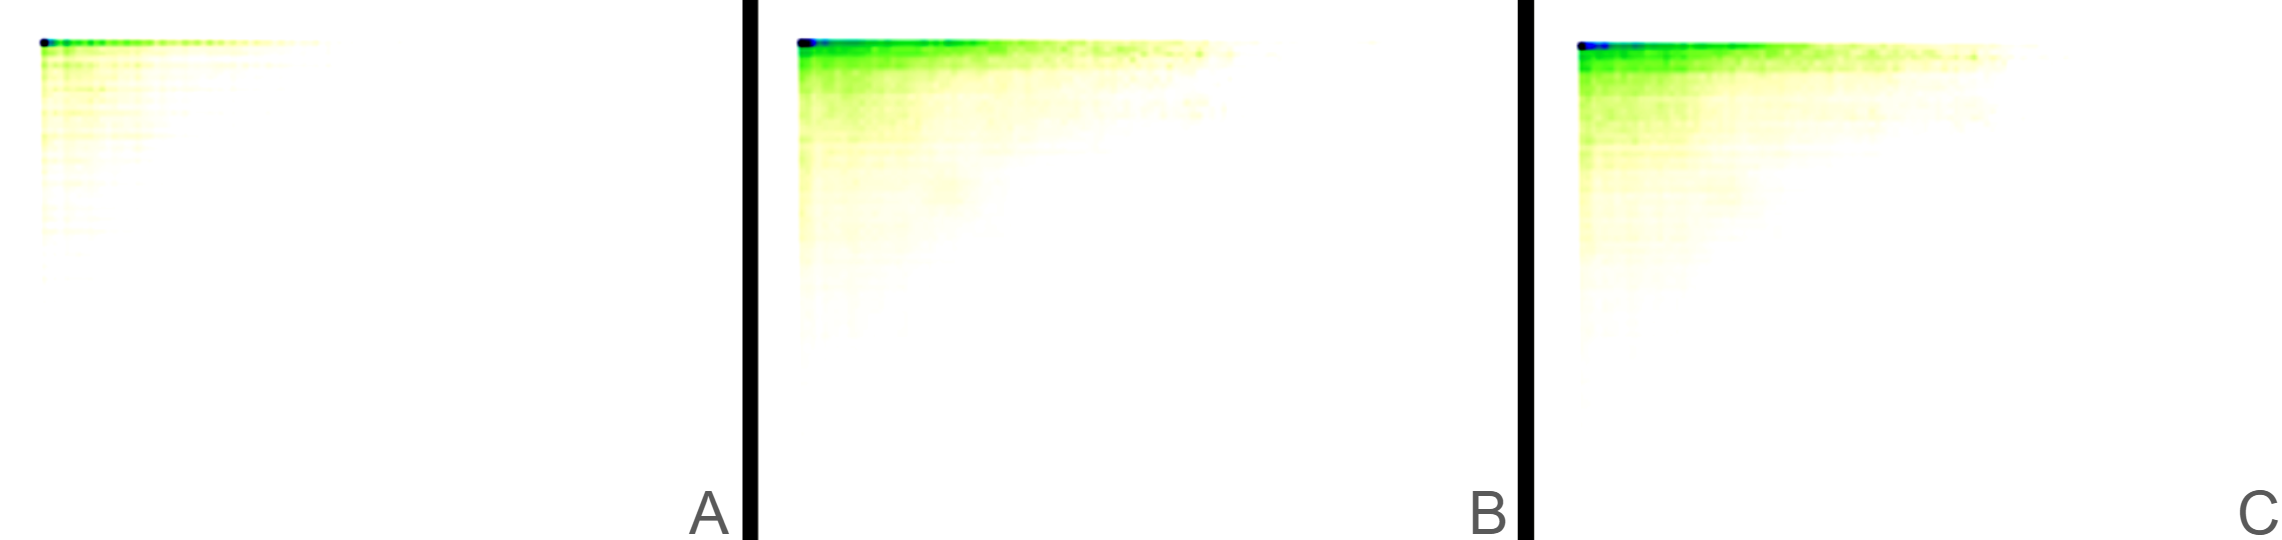
\includegraphics[width=0.92\textwidth]{figuras/xai.png}
    \fautor
\end{figure}

For Type classification, attributions often concentrate on structural bands,
indentation regions, and delimiter patterns. This is consistent with the idea
that file roles have visual structure. For Project classification, attributions
may highlight repository-specific conventions, headers, generated sections, or
boilerplate. For Author classification, attributions are more diffuse, suggesting
that stylistic signals are distributed and harder to localize.

These findings are valuable but also cautionary. If a Project classifier relies
heavily on boilerplate, it may not generalize to repositories with different
templates. If an Author classifier learns bot-generated patterns, it may not
represent human style. Explainability therefore serves as a check on the method,
not only as a defence of it.

\section{Study 3: Paired Anonymization Ablation}
\label{sec:study3-anonymization}

Because anonymization strips the lexical layer, the approach can be applied to
code that cannot leave an organization; the claim that it preserves predictive
utility therefore carries a large share of the proposal. Until recently that claim rested on a single
uncontrolled comparison. This section reports a controlled experiment designed
to replace it. It is a first instalment of Activity A2 rather than its
completion; the remaining scope is stated at the end of the section and in
Chapter~\ref{chapter:research-plan}.

\subsection{Design}

The experiment relies on a property of the method that makes the comparison
unusually direct. Anonymization is a deterministic per-character map applied
at rendering time: it changes pixel intensities and leaves geometry untouched.
The same source file can therefore be rendered twice, producing two images with
identical dimensions, identical layout and identical label, differing only in
the intensity alphabet. Both renderings are produced in a single pass, so the
two datasets are paired instance by instance. The pairing licenses paired
statistical tests, which are more sensitive than comparing two independent
runs.

The corpus is a large private enterprise system, a more recent version of one of
the projects used in the first study. Files were selected by extension, and only
textual source formats were read. Classes were defined by naming convention:
first by the suffix of the class name, and, when no suffix matched, by the
package the file belongs to. Keeping only classes with at least 300 examples and
capping each at 1,000 gives twelve classes and 10,927 paired minimaps, of which
10,923 pairs were usable. Descriptors are the same 59-bin LBP histograms used in
the first study.

The evaluation separates two questions that are routinely treated as one. The
first is whether any difference is detectable, and is answered by a paired
$t$-test over the cross-validation folds and by McNemar's test over paired
per-instance predictions \cite{mcnemar1947note}. The second is whether the
difference is small enough to be irrelevant, and is answered by two one-sided
tests of equivalence against a margin fixed before the experiment was run
\cite{schuirmann1987comparison}. The distinction matters: a non-significant
difference does not establish equivalence, since it may reflect nothing more
than lack of power. The equivalence margin was set at two percentage points of
accuracy. Both representations are evaluated on exactly the same splits of a
ten-times repeated five-fold stratified cross-validation, and the $t$-test uses
the correction of Nadeau and Bengio \cite{nadeau2003inference}, because folds of
a repeated cross-validation share training data and the uncorrected test is
anti-conservative.

\subsection{Results}

Table~\ref{tab:a2-anonymization} reports the outcome over fifty folds.

\begin{table}[ht]
\centering
\caption{Paired anonymization ablation with Random Forest over LBP descriptors,
twelve classes and 10,923 paired minimaps, ten times five-fold stratified
cross-validation. The difference is the accuracy lost by anonymizing.}
\label{tab:a2-anonymization}
\begin{tabular}{lc}
\toprule
\textbf{Measure} & \textbf{Value} \\
\midrule
Accuracy, original rendering & 0.8015 $\pm$ 0.0069 \\
Accuracy, anonymized rendering & 0.8076 $\pm$ 0.0063 \\
Difference (original $-$ anonymized) & $-$0.0060 \\
95\% confidence interval & [$-$0.0123, $+$0.0003] \\
Difference test (corrected paired $t$) & $p = 0.060$ \\
Equivalence within $\pm$0.02 (TOST) & $p = 2.4 \times 10^{-5}$ \\
\bottomrule
\end{tabular}
\fautor
\end{table}

Anonymization did not cost accuracy. The point estimate favours the anonymized
representation by 0.6 percentage points, and the confidence interval places the
largest loss compatible with the data at 0.0003, that is, at essentially zero.
The equivalence test rejects the hypothesis of a difference larger than the
declared margin.

The two tests should be read together rather than in isolation. The difference
test alone would support only the weak statement that no difference was
detected, at $p = 0.060$. The equivalence test supports the stronger and more
useful statement that the difference is bounded below the margin. McNemar's test
does find a detectable difference in six of the ten repetitions, and its
direction is consistent: across all repetitions, 5,239 instances were classified
correctly only by the anonymized representation against 4,580 only by the
original one. The result is therefore not that the two representations are
indistinguishable, but that the difference between them is small and, in this
setting, slightly favourable to anonymization.

A plausible explanation is that anonymization acts as a filter rather than only
as a loss. Collapsing letters and digits onto three intensities removes lexical
variation that a texture descriptor cannot exploit anyway, leaving the
structural skeleton more salient. The measurement in the next subsection
supports this reading.

\subsection{What the Transformation Removes}

The effect of anonymization on the representation can be quantified directly,
without training anything, because the map is deterministic. Measured over 12.3
million characters of the same corpus, the alphabet contracts from 152 to 37
distinct intensities and the entropy per pixel falls from 5.444 to 2.358 bits, a
reduction of 56.7\%. Only 25.9\% of characters survive unchanged, and those are
exactly the symbol classes: punctuation, delimiters and operators. The reduction
is uneven across file types, from 62.6\% for Java sources down to 48.0\% for SVG
files.

Read together, the two measurements say something that neither says alone: more
than half of the information carried by each pixel is discarded, and predictive
accuracy does not fall. That combination is evidence for the claim on which the
proposal rests, namely that the discriminative signal in a minimap is structural
rather than lexical. It also explains why the surviving 25.9\% is sufficient,
since block structure and layout are carried by punctuation and indentation.

\subsection{Scope of This Result}

Two boundaries must be respected when reading it. The evidence covers one
software system, so it establishes that anonymization can be cost-free, not that
it always is. And it covers one descriptor and one classifier family: Local
Binary Patterns describe local intensity relations, and may be constitutionally
blind to precisely the information that anonymization removes. A convolutional
model, which learns its own filters, could exploit lexical intensity differences
that LBP ignores, so this result does not transfer automatically to the
large-scale study of Section~\ref{sec:study2}. Extending the same protocol to
open-source corpora, to deep models, and to the Project and Author objectives is
the remainder of Activity A2.

\section{Artifact and Tool Results}

In addition to the two empirical studies, this work produced MinimapSignatures,
a multi-IDE tool ecosystem composed of a FastAPI/PyTorch inference backend, a
Visual Studio Code extension, and an IntelliJ IDEA plugin
\cite{gebara2026minimapsignatures}. The workflow was validated end-to-end: each
plugin generates an anonymized 128 by 128 minimap locally, submits it to the
backend, and displays ranked predictions for the Type, Project, and Author
targets. A fourth response target (quality) is a placeholder and currently
returns mock data; no model has been trained for it.

With this line of work, the thesis is no longer limited to a dataset-and-model
comparison; it also investigates how minimap analysis can become usable
infrastructure for software-engineering workflows. No user study
has been conducted yet, so the evaluation remains functional and
integration-oriented. The architecture, the deployed multitask model, the
current capture limits, and the validation status are detailed in
Chapter~\ref{chapter:tool-support}.

\section{Consolidated Evidence}

Table~\ref{tab:preliminary-evidence} summarizes the evidence produced so far and
how it supports the research questions.

\begin{table}[ht]
\centering
\caption{Preliminary evidence and relation to research questions.}
\label{tab:preliminary-evidence}
\begin{tabular}{p{0.24\textwidth}p{0.43\textwidth}p{0.18\textwidth}}
\toprule
\textbf{Evidence} & \textbf{Main finding} & \textbf{Related RQs} \\
\midrule
LBP study & Minimap texture supports software-feature classification with Random Forest near 93\% accuracy. & RQ1, RQ2 \\
Fixed-size comparison & 128 by 128 minimaps remain competitive with variable-size minimaps. & RQ1, RQ2 \\
Large-scale dataset & Minimap learning scales to 685,906 images from 100 projects and 10 languages. & RQ1 \\
Deep learning results & EfficientNet-B0 pretrained reaches strong validation results for Type, Project, and Author. & RQ1, RQ2 \\
Integrated Gradients & Different objectives rely on different visual regions and patterns. & RQ3 \\
MinimapSignatures & IDE plugins and backend validate an end-to-end tool workflow. & RQ5 \\
\bottomrule
\end{tabular}
\fautor
\end{table}

The evidence supports continuing the doctoral research, but it also defines the
remaining challenges. The next phase must deepen the evaluation of
anonymization, improve imbalance-aware learning, refine dataset splits, extend
the task set toward quality and architectural analysis, and evaluate the tool
with developers or realistic development scenarios.

\section{Interpretation by Research Question}

The preliminary studies already provide partial answers to the research
questions stated in the Introduction.

\subsection{RQ1: Discriminative Structural Cues}

The LBP study and the large-scale deep learning study both support the idea that
minimaps preserve discriminative structural cues. In the first study, the
success of Random Forest over LBP histograms indicates that texture-level
information is meaningful. In the second study, the strong Type classification
results indicate that fixed-size minimaps preserve enough information to
distinguish many artifact categories across a much larger corpus. Together,
these results support the representational premise of the work: the
two-dimensional layout of source files carries a signal that survives both
compression to 128 by 128 pixels and lexical suppression, and that would not be
directly visible to models consuming code as a one-dimensional sequence.

However, RQ1 is not fully answered. The current evidence is strongest for the
datasets already used. Future work must evaluate additional repositories,
stronger splits, and quality-related tasks. It must also examine which classes
are consistently difficult and whether failures are due to representation loss,
label ambiguity, or insufficient samples.

\subsection{RQ2: Handcrafted and Learned Representations}

The first study shows that handcrafted texture descriptors are a viable
baseline. The second study shows that deep models can operate directly on
minimap images at scale. The comparison suggests that handcrafted descriptors
are useful for simpler settings, while learned representations become important
when the dataset is larger, more imbalanced, and more heterogeneous.

The remaining work should compare these pipelines under the same dataset
conditions. For example, LBP histograms can be computed for the large-scale
dataset and compared with deep models under identical splits. This would make
the answer to RQ2 more precise.

\subsection{RQ3: Visual Evidence and Explainability}

Integrated Gradients provides an initial answer to RQ3. The attribution maps
suggest that models use structural bands, boilerplate regions, and diffuse style
patterns depending on the objective. This supports the claim that predictions
are not arbitrary, but it also reveals risks. If a model depends too strongly on
headers or generated sections, then its performance may reflect dataset
artifacts rather than genuine software structure.

Future work must make this analysis more systematic. Instead of inspecting only
representative examples, the thesis should aggregate attribution statistics,
compare attribution patterns across classes, and perform ablation experiments
that remove or mask salient regions.

\subsection{RQ4: Anonymization}

The paired ablation of Section~\ref{sec:study3-anonymization} answers this
question directly for one system. Over twelve classes and 10,923 paired
minimaps, anonymization did not reduce accuracy: the difference was $-0.0060$ in
favour of the anonymized representation, with a 95\% confidence interval whose
upper bound is 0.0003, and equivalence within two percentage points holds at
$p = 2.4 \times 10^{-5}$. The result is reinforced by the measurement of the
transformation itself, which discards 56.7\% of the entropy per pixel while
leaving accuracy intact. An earlier comparison made during the first study
pointed in the same direction, with average F1-score falling from 0.83 to 0.82
for an SVM over ten classes \cite{gebara2025iwssip}, though that figure came
from a single uncontrolled run.

This evidence matters for two reasons.

First, it indicates that the discriminative signal resides in structural
features such as indentation patterns, operator density, punctuation layout,
and block organization, rather than in identifier names or literal values. The
model does not appear to need lexical content to distinguish file types,
project origins, or authorship styles.

Second, it supports the industrial motivation developed in
Chapter~\ref{chapter:foundations}: if anonymization preserves utility, an
organization can submit anonymized minimaps to an external analysis service
while the business logic embedded in the lexical layer stays local.

The Author objective matters here. Style remains identifiable after full
lexical suppression, which is direct evidence that the model operates on
structural patterns; if author identification depended on lexical content,
anonymization would have eliminated it.

A formal ablation study is still required. The thesis should repeat the
comparison under documented conditions, cover multiple suppression levels,
measure degradation curves, and characterize what remains inferable from
anonymized minimaps under each strategy (Activity A2 in
Chapter~\ref{chapter:research-plan}).

\subsection{RQ5: IDE Integration}

MinimapSignatures provides an initial answer to RQ5 by showing that minimap
analysis can be integrated into Visual Studio Code and IntelliJ IDEA. The
functional validation confirms that the technical workflow is feasible.

However, developer usefulness remains open. The current prototype shows that
predictions can be delivered inside IDEs, but it does not prove that developers
benefit from them. Future work must evaluate whether the feedback is
understandable, whether explanations increase trust, and whether multi-file
analysis is more useful than single-file prediction.

\section{Limitations of the Current Evidence}

The current evidence has several limitations. First, the first study uses a
limited dataset compared with the later corpus. Its results are valuable as
proof of feasibility, but they should not be generalized beyond the evaluated
setting without further experiments.

Second, the large-scale study is affected by class imbalance. Strong accuracy
and ROC-AUC values show that the models learn substantial signal, but they do
not guarantee equally strong behavior for minority classes. Macro-F1, per-class
recall, and confusion matrices must be emphasized in the thesis.

Third, the Author objective must be interpreted carefully. Labels may reflect
last committers, bots, project maintainers, or generated artifacts, which
introduces noise. Methodologically, the objective serves as a probe: it tests
whether style-related structural patterns survive anonymization. In this role it
is valuable. However, the objective is not presented as a deployment-ready
author identification tool, and the thesis should be explicit about this
distinction.

Fourth, the current tool evaluation is functional. It confirms that the
architecture works, but it does not measure usability, usefulness, or impact on
developer productivity. This distinction must be preserved in the thesis.

Finally, the current studies focus mostly on classification. The most valuable
software-engineering applications may require ranking, anomaly detection,
clustering, explanation, or integration with other signals. These directions
remain to be explored.

\section{Implications for the Thesis}

The preliminary results shape the final thesis in a concrete way. The thesis
does not need to prove from scratch that minimaps contain information; the early
studies already support that claim. Instead, the thesis must characterize that
information: how far it generalizes, how it can be interpreted, and what it is
useful for.

This shifts the emphasis from simple feasibility to disciplined evaluation. The
next experiments should ask harder questions: whether the representation
generalizes across repositories, whether minority classes are handled fairly,
whether anonymization is strong enough, whether explanations reveal meaningful
evidence, and whether developers can use the feedback in realistic tasks.

The final thesis should therefore be organized around a progression:
representation, evidence, interpretation, and operationalization. The current
chapter provides the evidence base for that progression.
